\chapter{Αρχιτεκτονική Lambda}
Ένα από τα πιο σύνθετα προβλήματα που χρειάζεται να αντιμετωπίζουν τα Big Data συστήματα είναι η εύρεση λύσης/απάντησης σε πραγματικό χρόνο.Κατά την αρχική τους σχεδίαση, δεν υπήρχε καμία πρόβλεψη για την αντιμετώπιση αυτού του είδους των προβλημάτων και φαινόταν έξω από την σφαίρα των δυνατοτήτων τους. Με την υποστήριξη και την ανάπτυξη που έλαβαν τα χρόνια μετά την εμφάνιση τους, βοήθησαν να αναπτυχθούν και να εδραιωθούν σε όλο και περισσότερους τομείς της πληροφορικής. Ο τομέας των real-time analytics αποδείχθηκε ένα αρκετά μεγάλο πρόβλημα, λόγω του όγκου της πληροφορίας που αποθηκεύεται σε ένα τέτοιο σύστημα. Η λύση ακόμα δεν έχει δοθεί από ένα μόνο συγκεκριμένο σύστημα αλλά έχει περιγραφτεί μια αρχιτεκτονική συστημάτων που παράγει το σωστό αποτέλεσμα, με μερικούς περιορισμούς.Η αρχιτεκτονική αυτή ονομάζεται Lambda και οι βασικές της αρχές θα αναλυθούν σε αυτό το κεφάλαιο.

\section{Επίπεδα}
Η βασική ιδέα της αρχιτεκτονικής Lambda είναι τα επίπεδα. Κάθε Big Data σύστημα που την εφαρμόζει θα αποτελεί μια σειρά από επίπεδα όπου σε κάθε επίπεδο εφαρμόζετε διαφορετικό σύστημα. Όλα μαζί τα επίπεδα λειτουργούν ως ένα ενιαίο real-time system.Το κάθε επίπεδο έχει διαφορετικό σκοπό και ο οποίος ενεργεί σε συνδυασμό με τα αποτελέσματα των επιπέδων κάτω από αυτό.Στην πολύ απλή τους μορφή τα επίπεδα είναι αυτά που φαίνονται στο σχήμα 1.1 .

\begin{figure}[t]
\caption{Επίπεδα της Αρχιτεκτονικής Lambda}
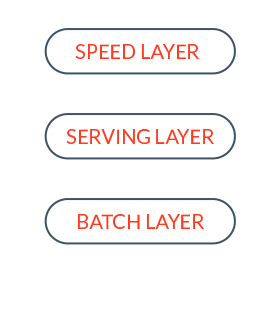
\includegraphics[width=8cm]{images/layers.png}
\centering
\end{figure}

\section{Query}
Αυτός ο πολύ απλός ορισμός των επιπέδων αρκεί, για αυτό το κεφάλαιο, για να γίνει κατανοητή η λειτουργία της Αρχιτεκτονικής Lambda. Όπως έχει αναφερθεί, το πρόβλημα που πρέπει να λυθεί είναι τα real-time analytics.Αυτό μπορεί να συνοψιστεί, για λόγους απλότητας, σε μια πρόταση ως εξής:
\begin{verbatim}
query = function(all data)
\end{verbatim}

Όπου \textit{query} είναι η ερώτηση που υποβάλετε στο σύστημα, η \textit{function} είναι η συνάρτηση υπολογισμού της απάντησης πάνω στα \textit{data}, όλα τα δεδομένα που έχει αποθηκευμένα το σύστημα εκείνη την χρονική στιγμή.
\newline
Στα περισσότερα Big Data συστήματα αυτός ο υπολογισμός θα απαιτούσε από μερικές ώρες μέχρι μερικές ημέρες, δεδομένου του μεγέθους που έχουν τα δεδομένα και την πολυπλοκότητα του υπολογισμού. Για να μπορέσει να απαντηθεί ένα τέτοιο ερώτημα σε real-time θα έπρεπε να χρησιμοποιηθούν τεράστιες υποδομές ηλεκτρονικών υπολογιστών και το κόστος, στις περισσότερες περιπτώσεις, για κάτι τέτοιο υπερβαίνει την αξία της απάντησης. Με την Αρχιτεκτονική Lambda αναμένετε η απάντηση να δοθεί σε μερικά δευτερόλεπτα έως λεπτά σε υποδομές πολύ μικρότερης κλίμακας και κόστους. 